\begin{subsectionframemod}{Performance Analysis}
    
    
    Il est impossible de comparer les performances sur différents ensembles de données.
    Cependant, il est possible de \alert{comparer les performances FSOD par rapport à une référence non few-shot}
    et de comparer cela sur plusieurs ensembles de données.

    \begin{figure}
        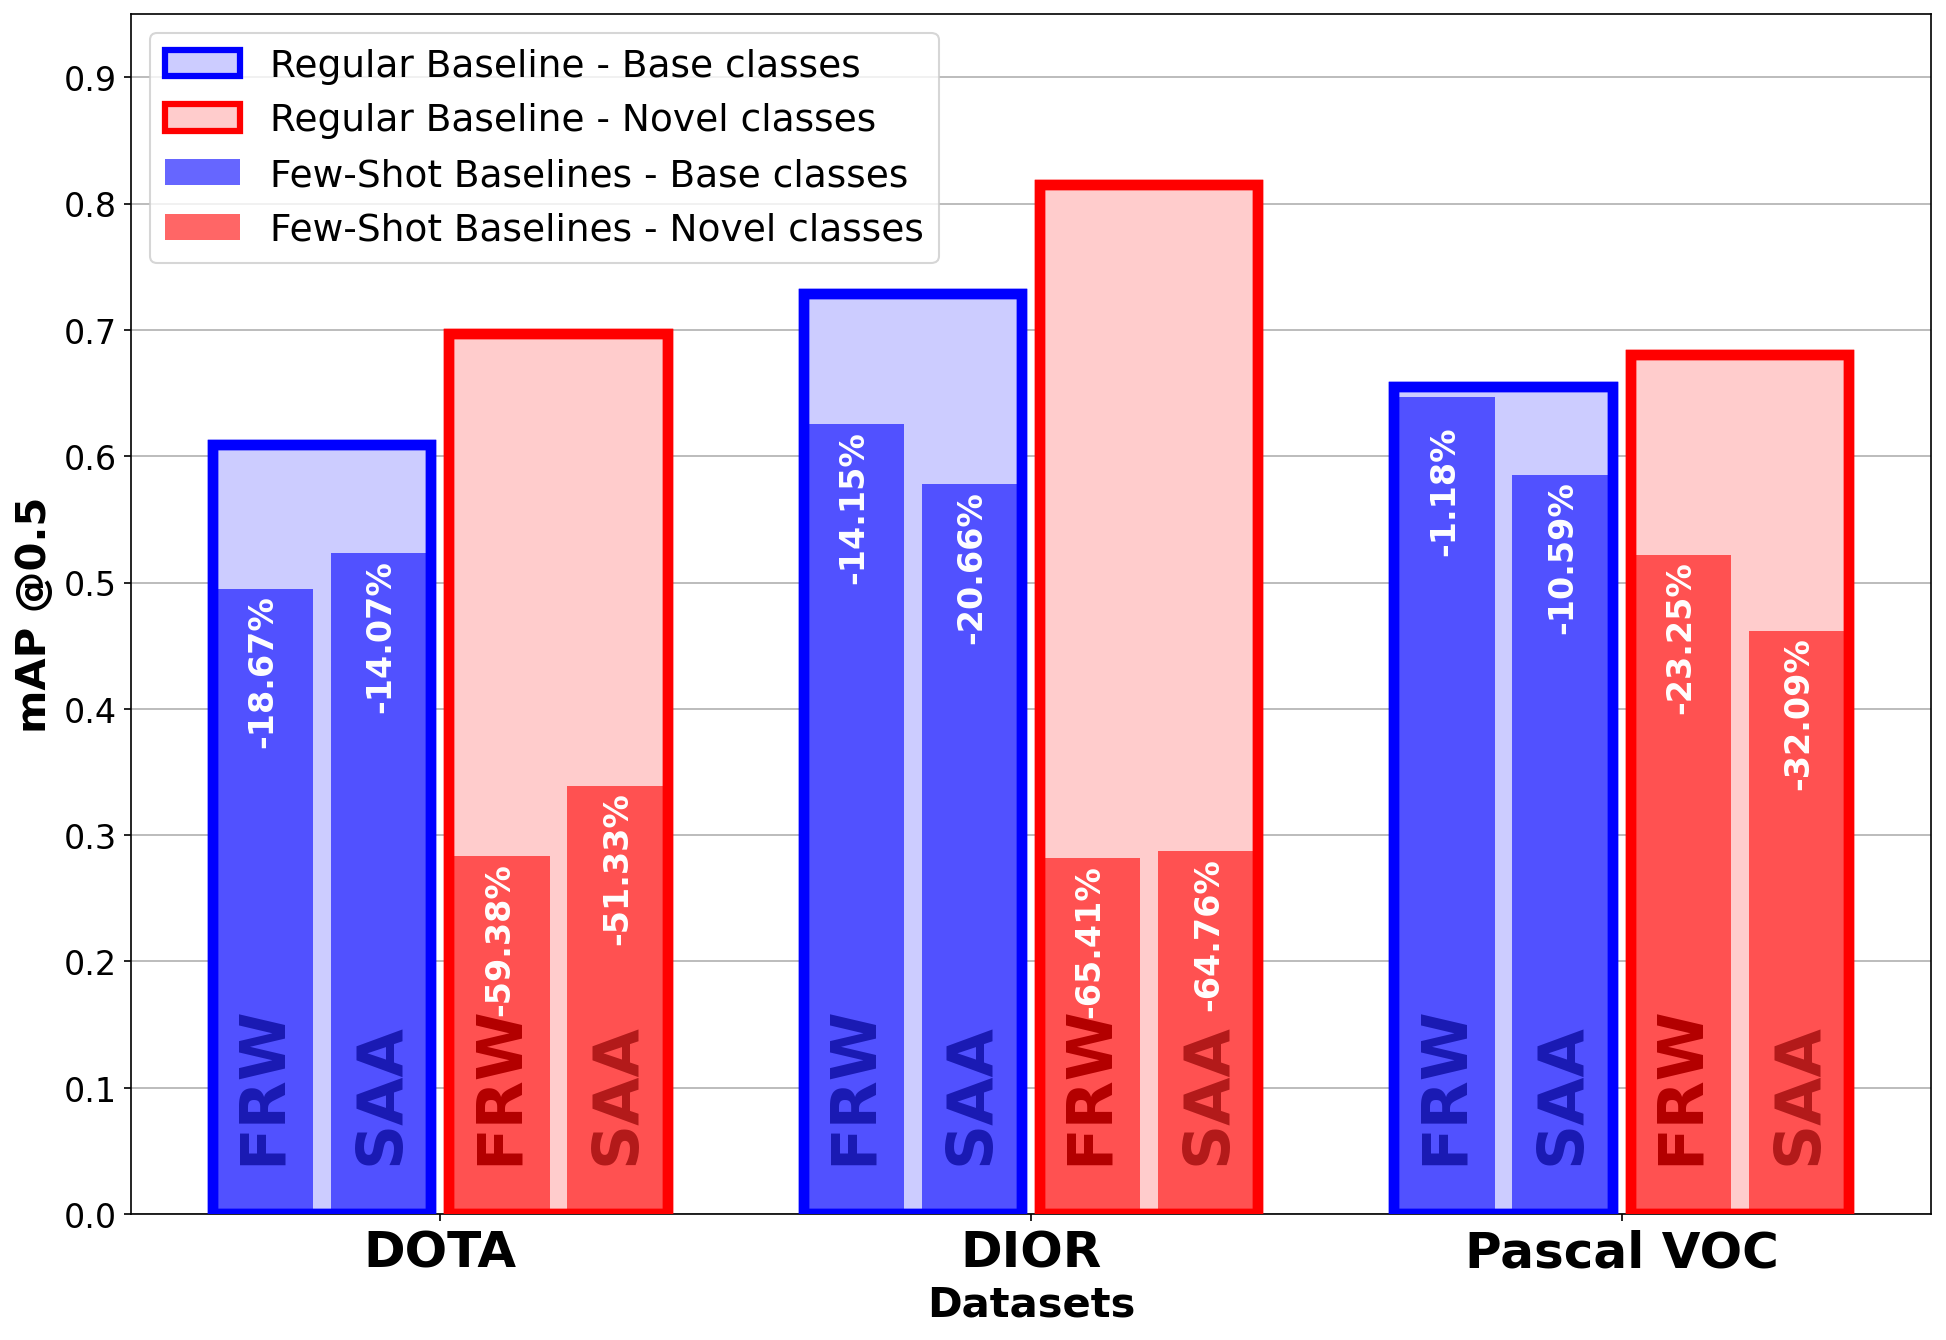
\includegraphics[width=0.8\textwidth]{Figures/dataset_comparison.png}
        \caption{Performances FSOD comparées sur DOTA, DIOR et Pascal VOC. (\cite{lejeune2022improving})}
    \end{figure}

\end{subsectionframemod}

\begin{subsectionframemod}{Performance Analysis}
    Les grandes différences de taille moyenne entre les classes suggèrent d'analyser les performances par classe.
    \alert{Corrélation claire entre la taille moyenne des classes et les performances} par rapport à la référence.
    \begin{figure}
        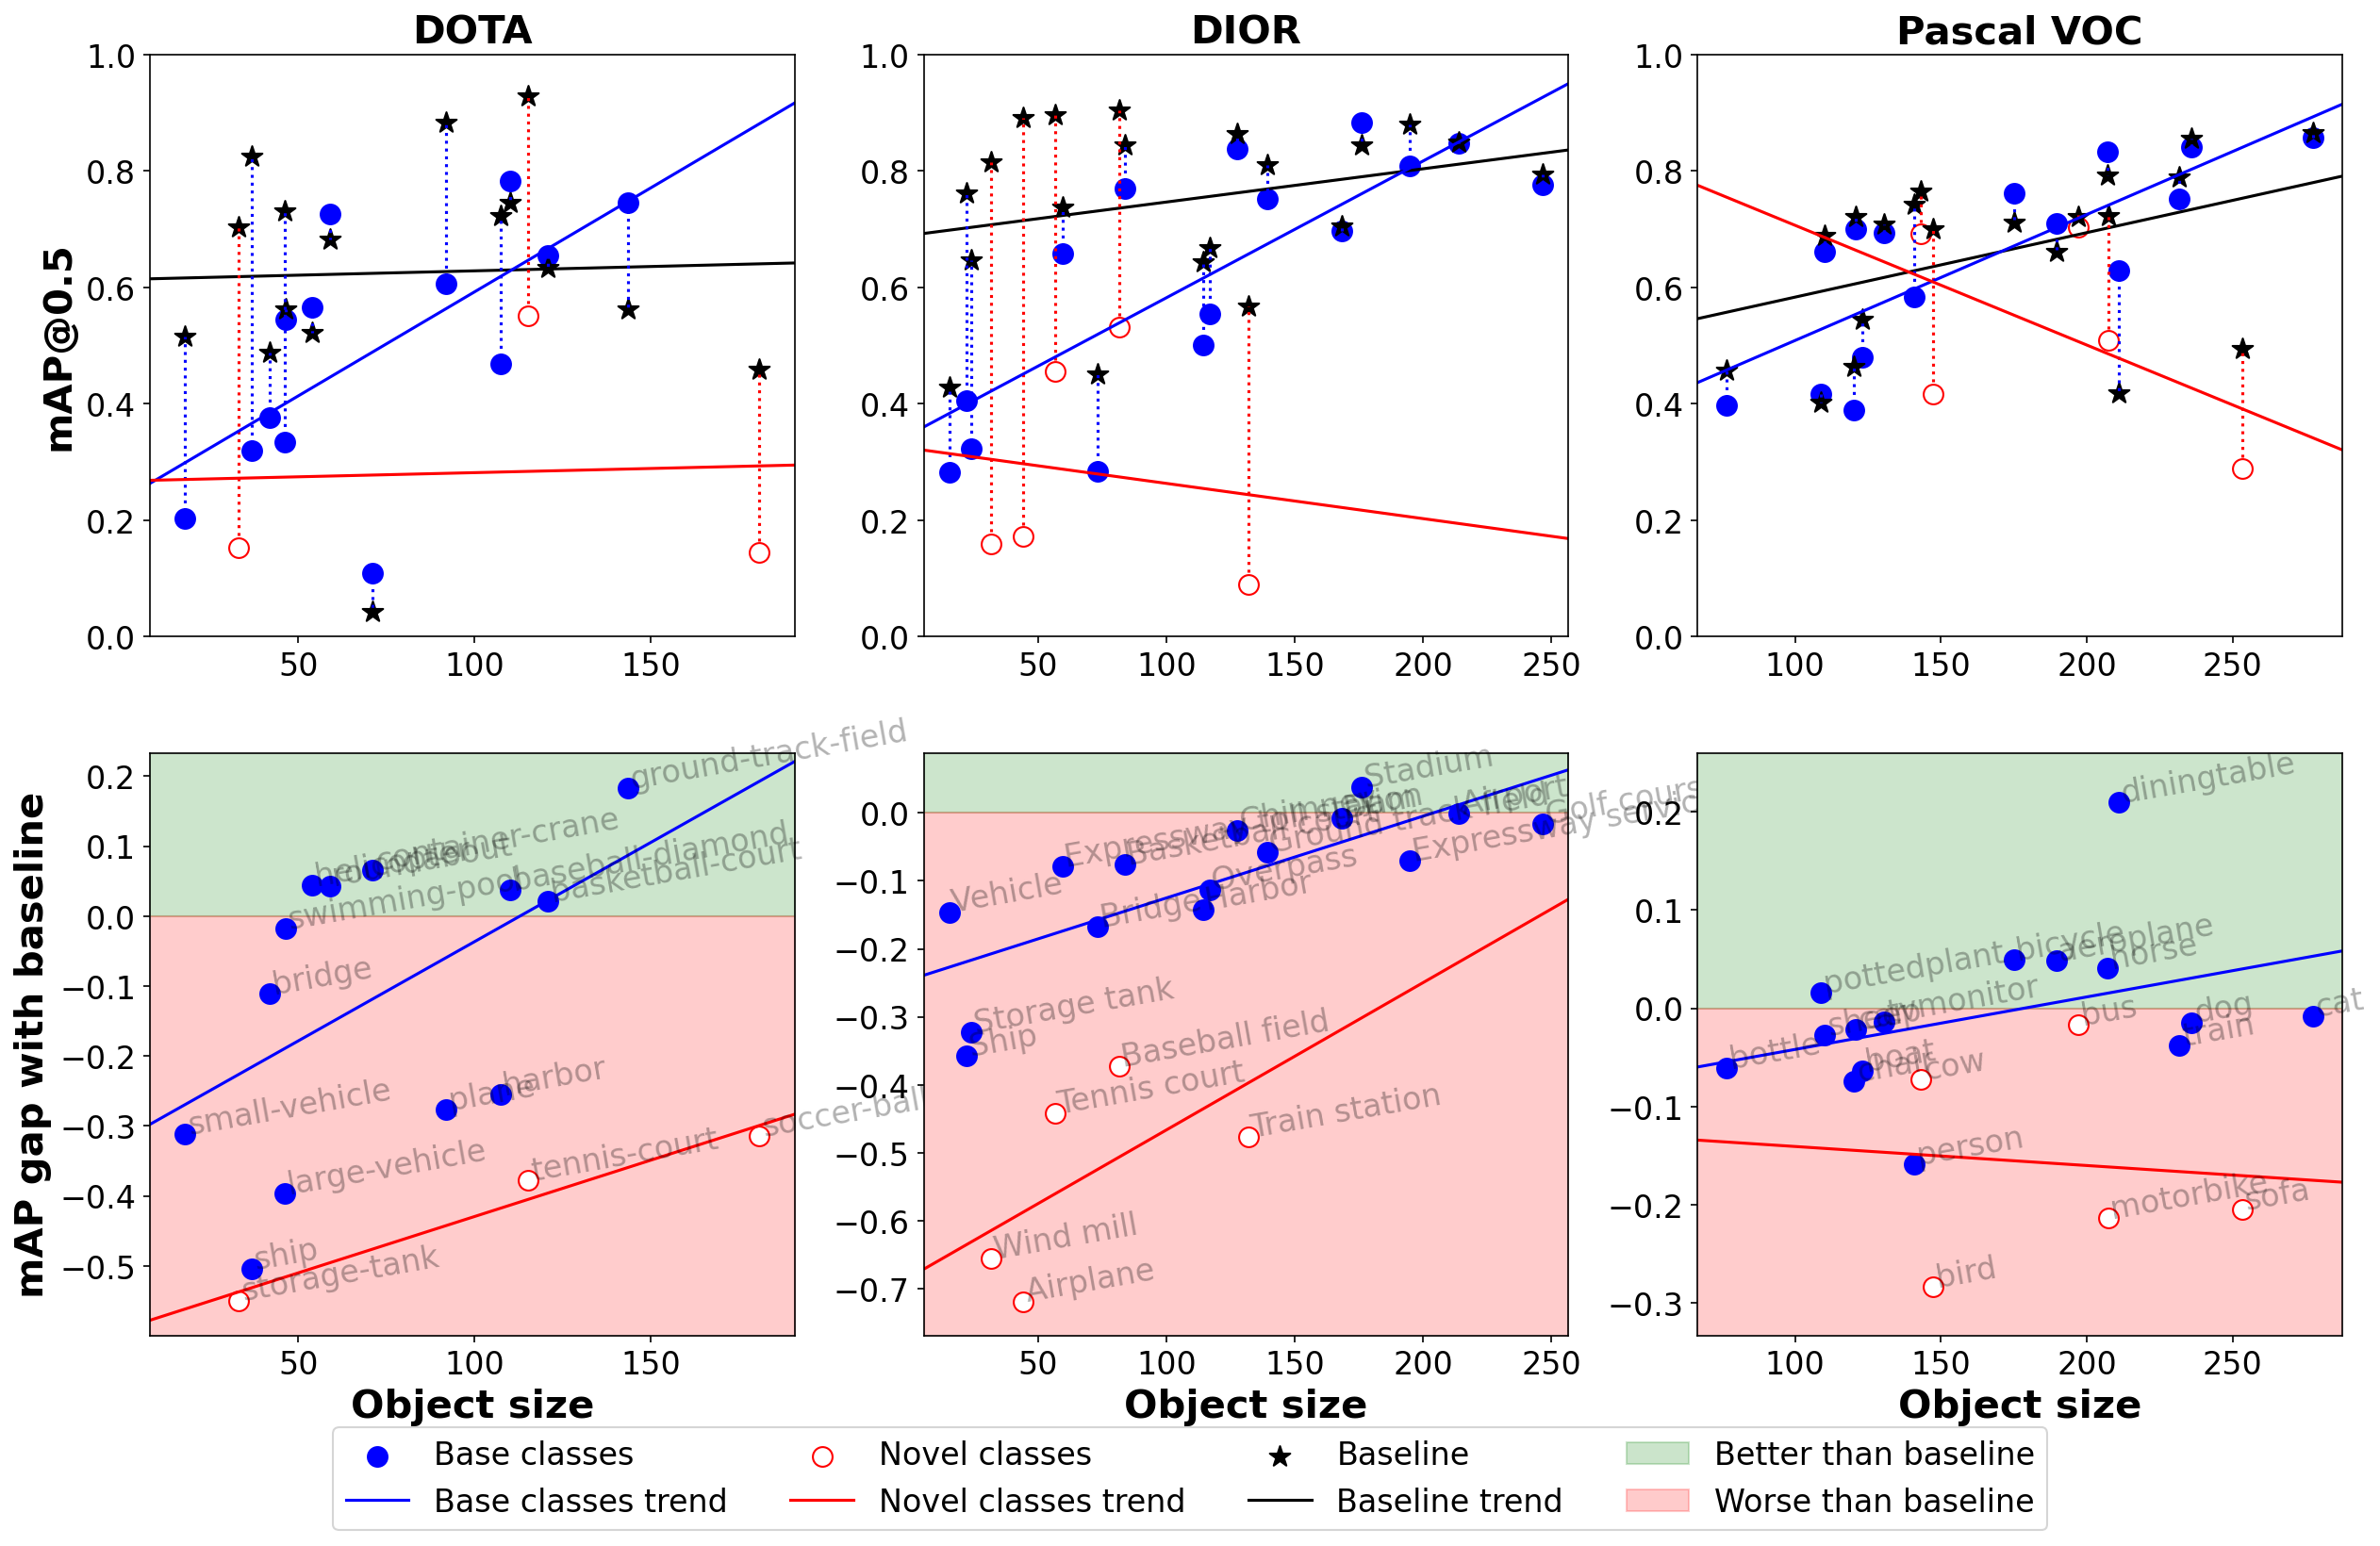
\includegraphics[width=0.85\textwidth]{Figures/performance_comparison.png}
    \caption{Analyse des performances par classe et comparaison avec la référence non few-shot sur DOTA, DIOR et Pascal VOC. (\cite{lejeune2022improving})}
    \end{figure}

\end{subsectionframemod}